%!TEX TS-program = ../make.zsh

\subsection{Simulating Shadowing Cables as Opaque Cylinders}
\label{sec:cables}

% https://github.com/fiedl/hole-ice-study/issues/35

% \cite{instrumentation}: In-ice cable cross section, with a nominal 46 mm diameter and mass of 2 kg/m.
The main cable of each detector string (figure \ref{fig:ahyoi7Ma}) allows to power the detector modules and to transfer data from the modules to the surface. The cable has a diameter of $46\mm$ \cite{instrumentation} and, as it is located in close proximity to the optical modules, shields the optical modules from a non-neglectable amount of incoming photons. The cable's mantle is black such that it will absorb photons rather than reflect them.

\begin{figure}[htbp]
  \subcaptionbox{Optical module deployment schematics. Image source:  \cite{instrumentation}}{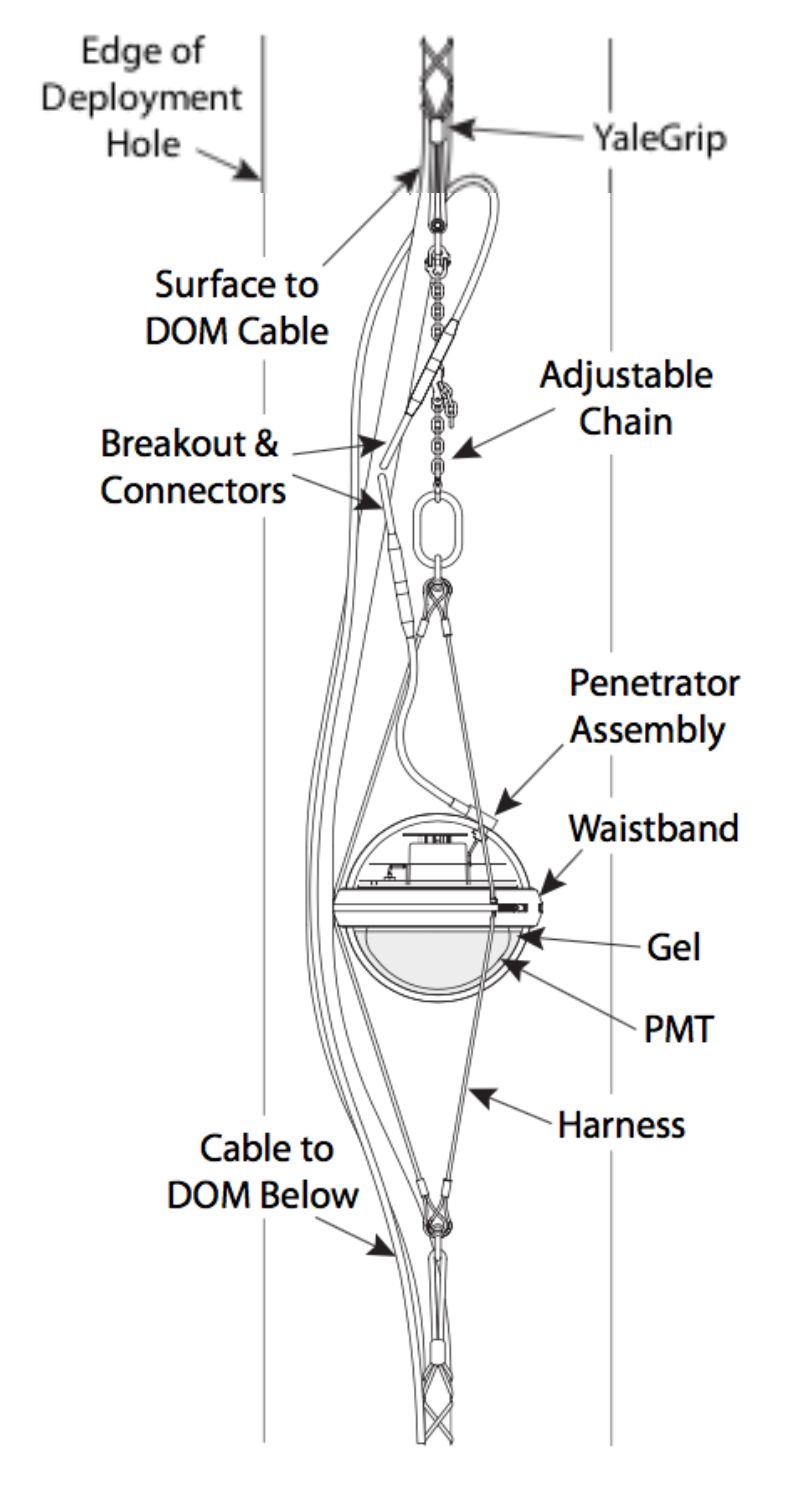
\includegraphics[width=0.25\textwidth]{img/dom-cable-instrumentation}}\hfill
  \subcaptionbox{Rendered image of the optical module and the main cable. Image source: \cite{gallerydomcloseup}}{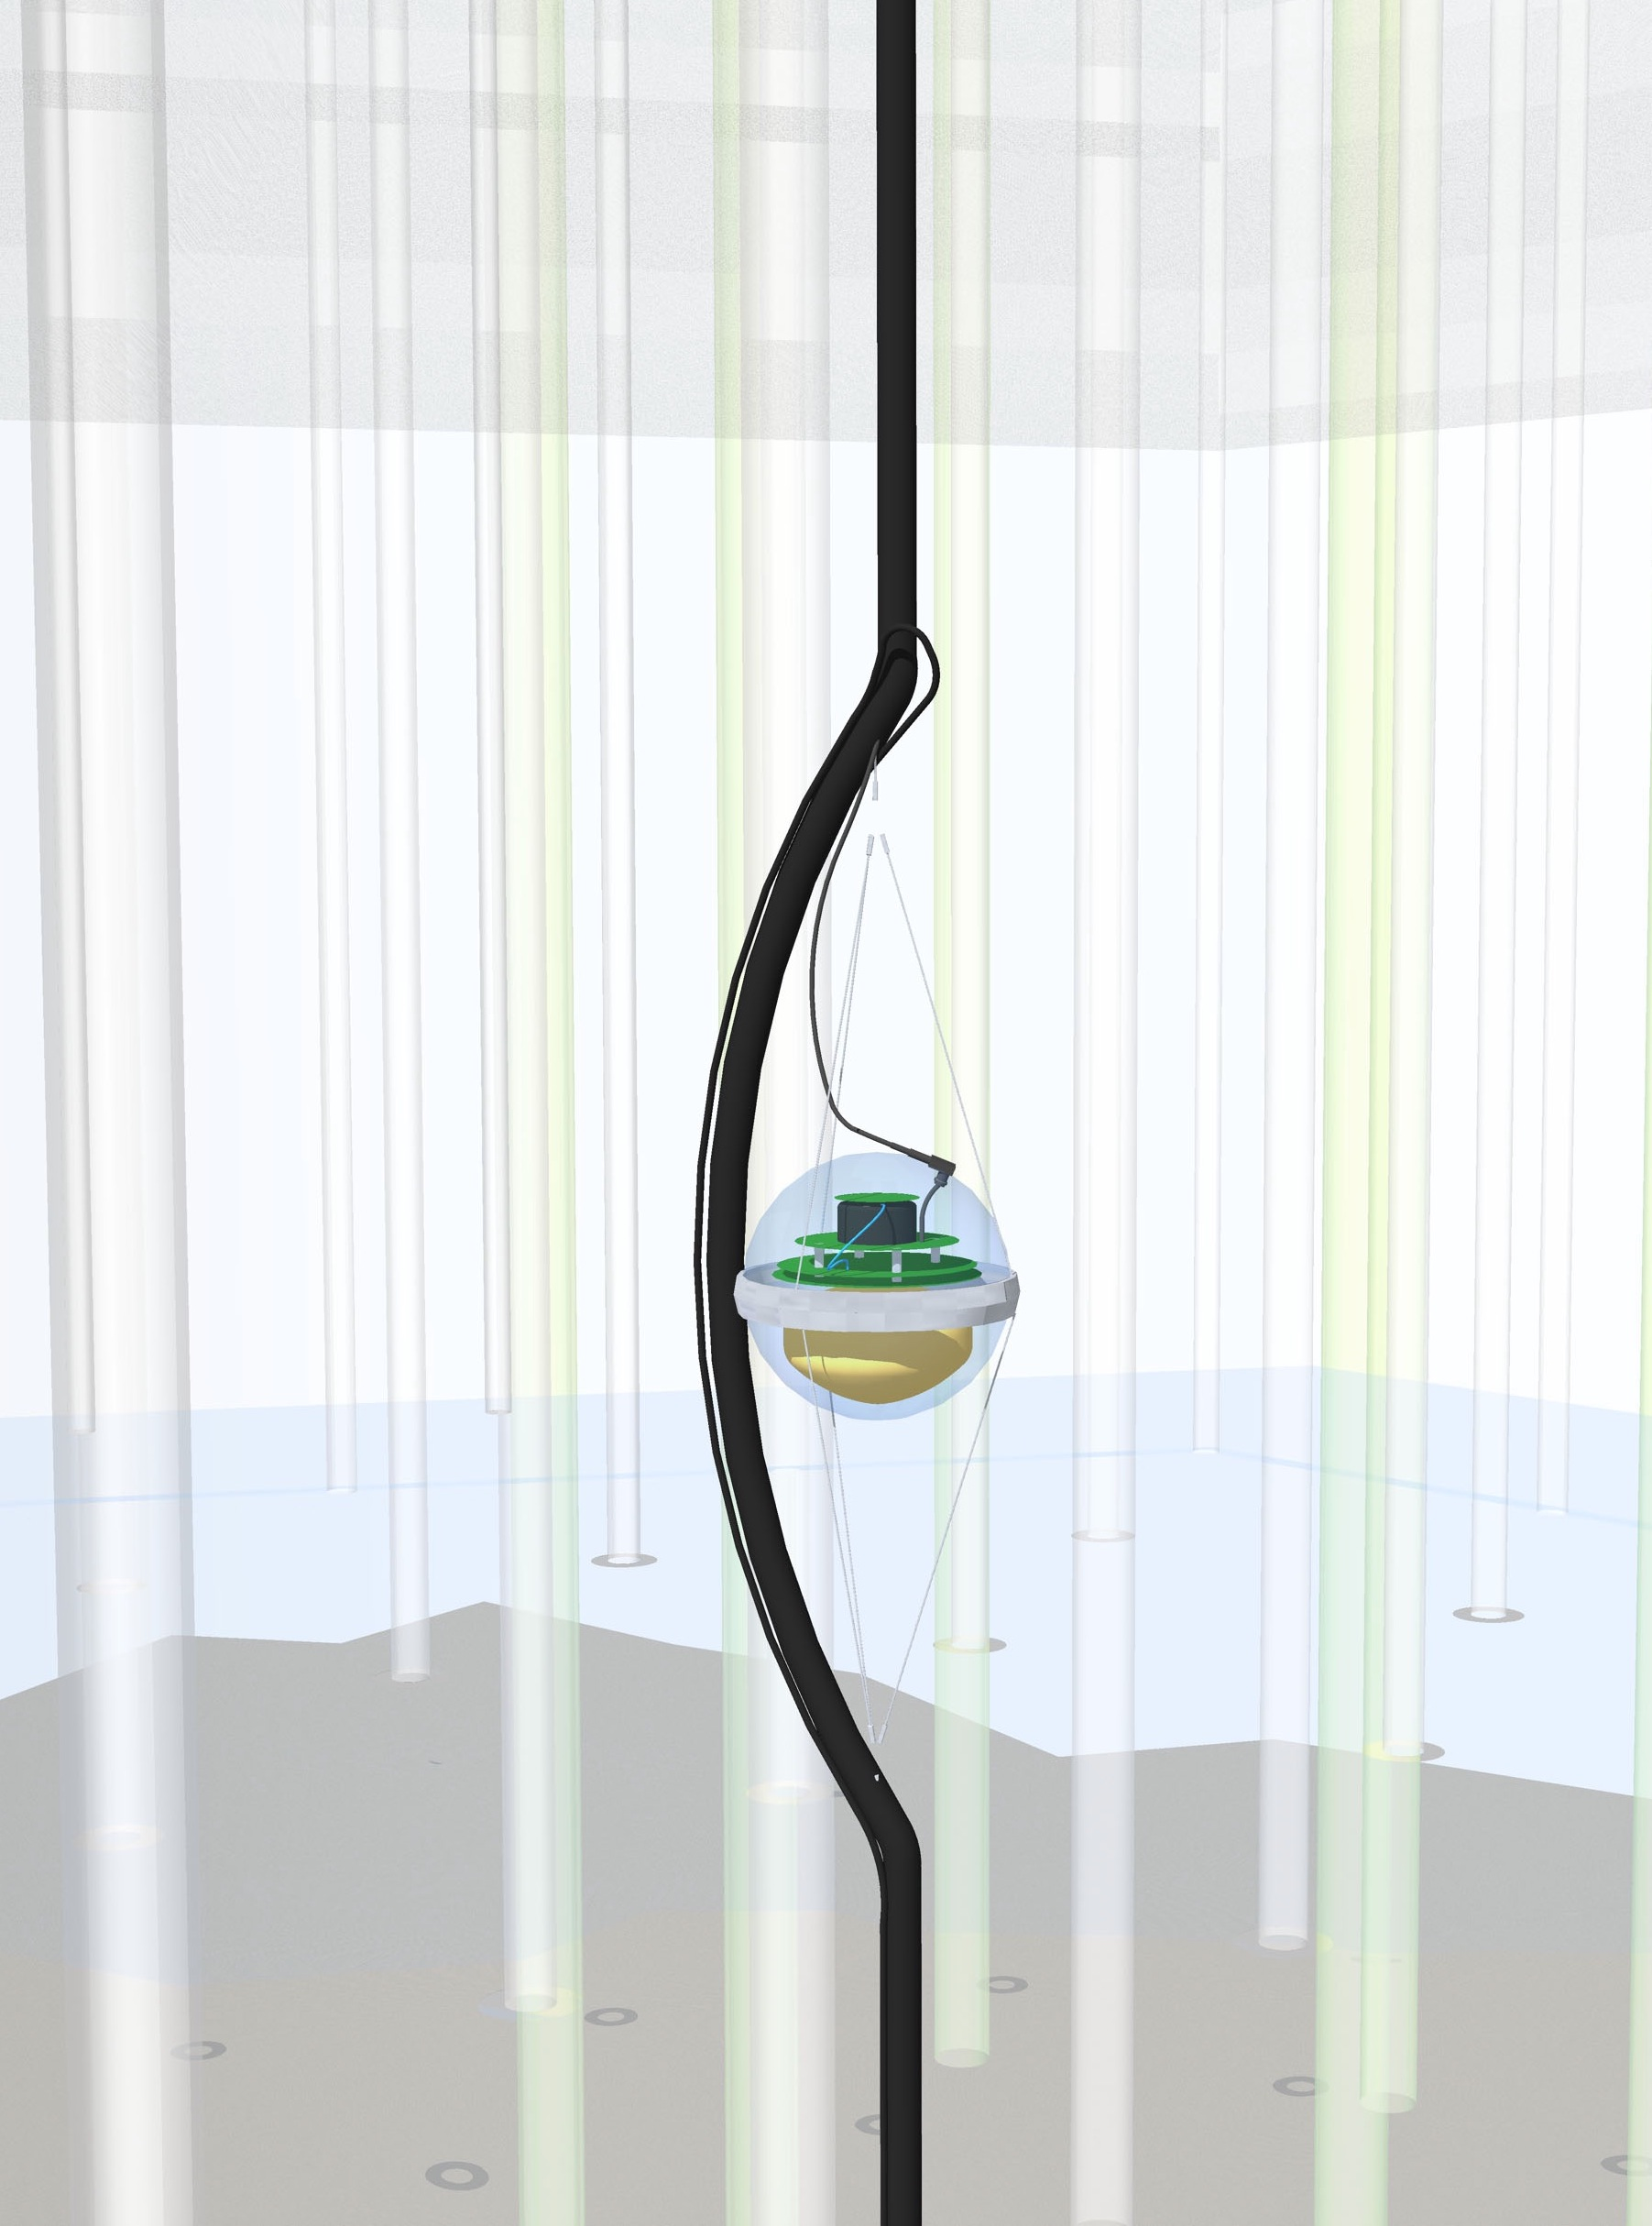
\includegraphics[width=0.35\textwidth]{img/DOMCloseUp-cropped-mirrored}}\hfill
  \subcaptionbox{Photo: Optical module deployment. Image source: \cite{publicgallerydomdeployment}}{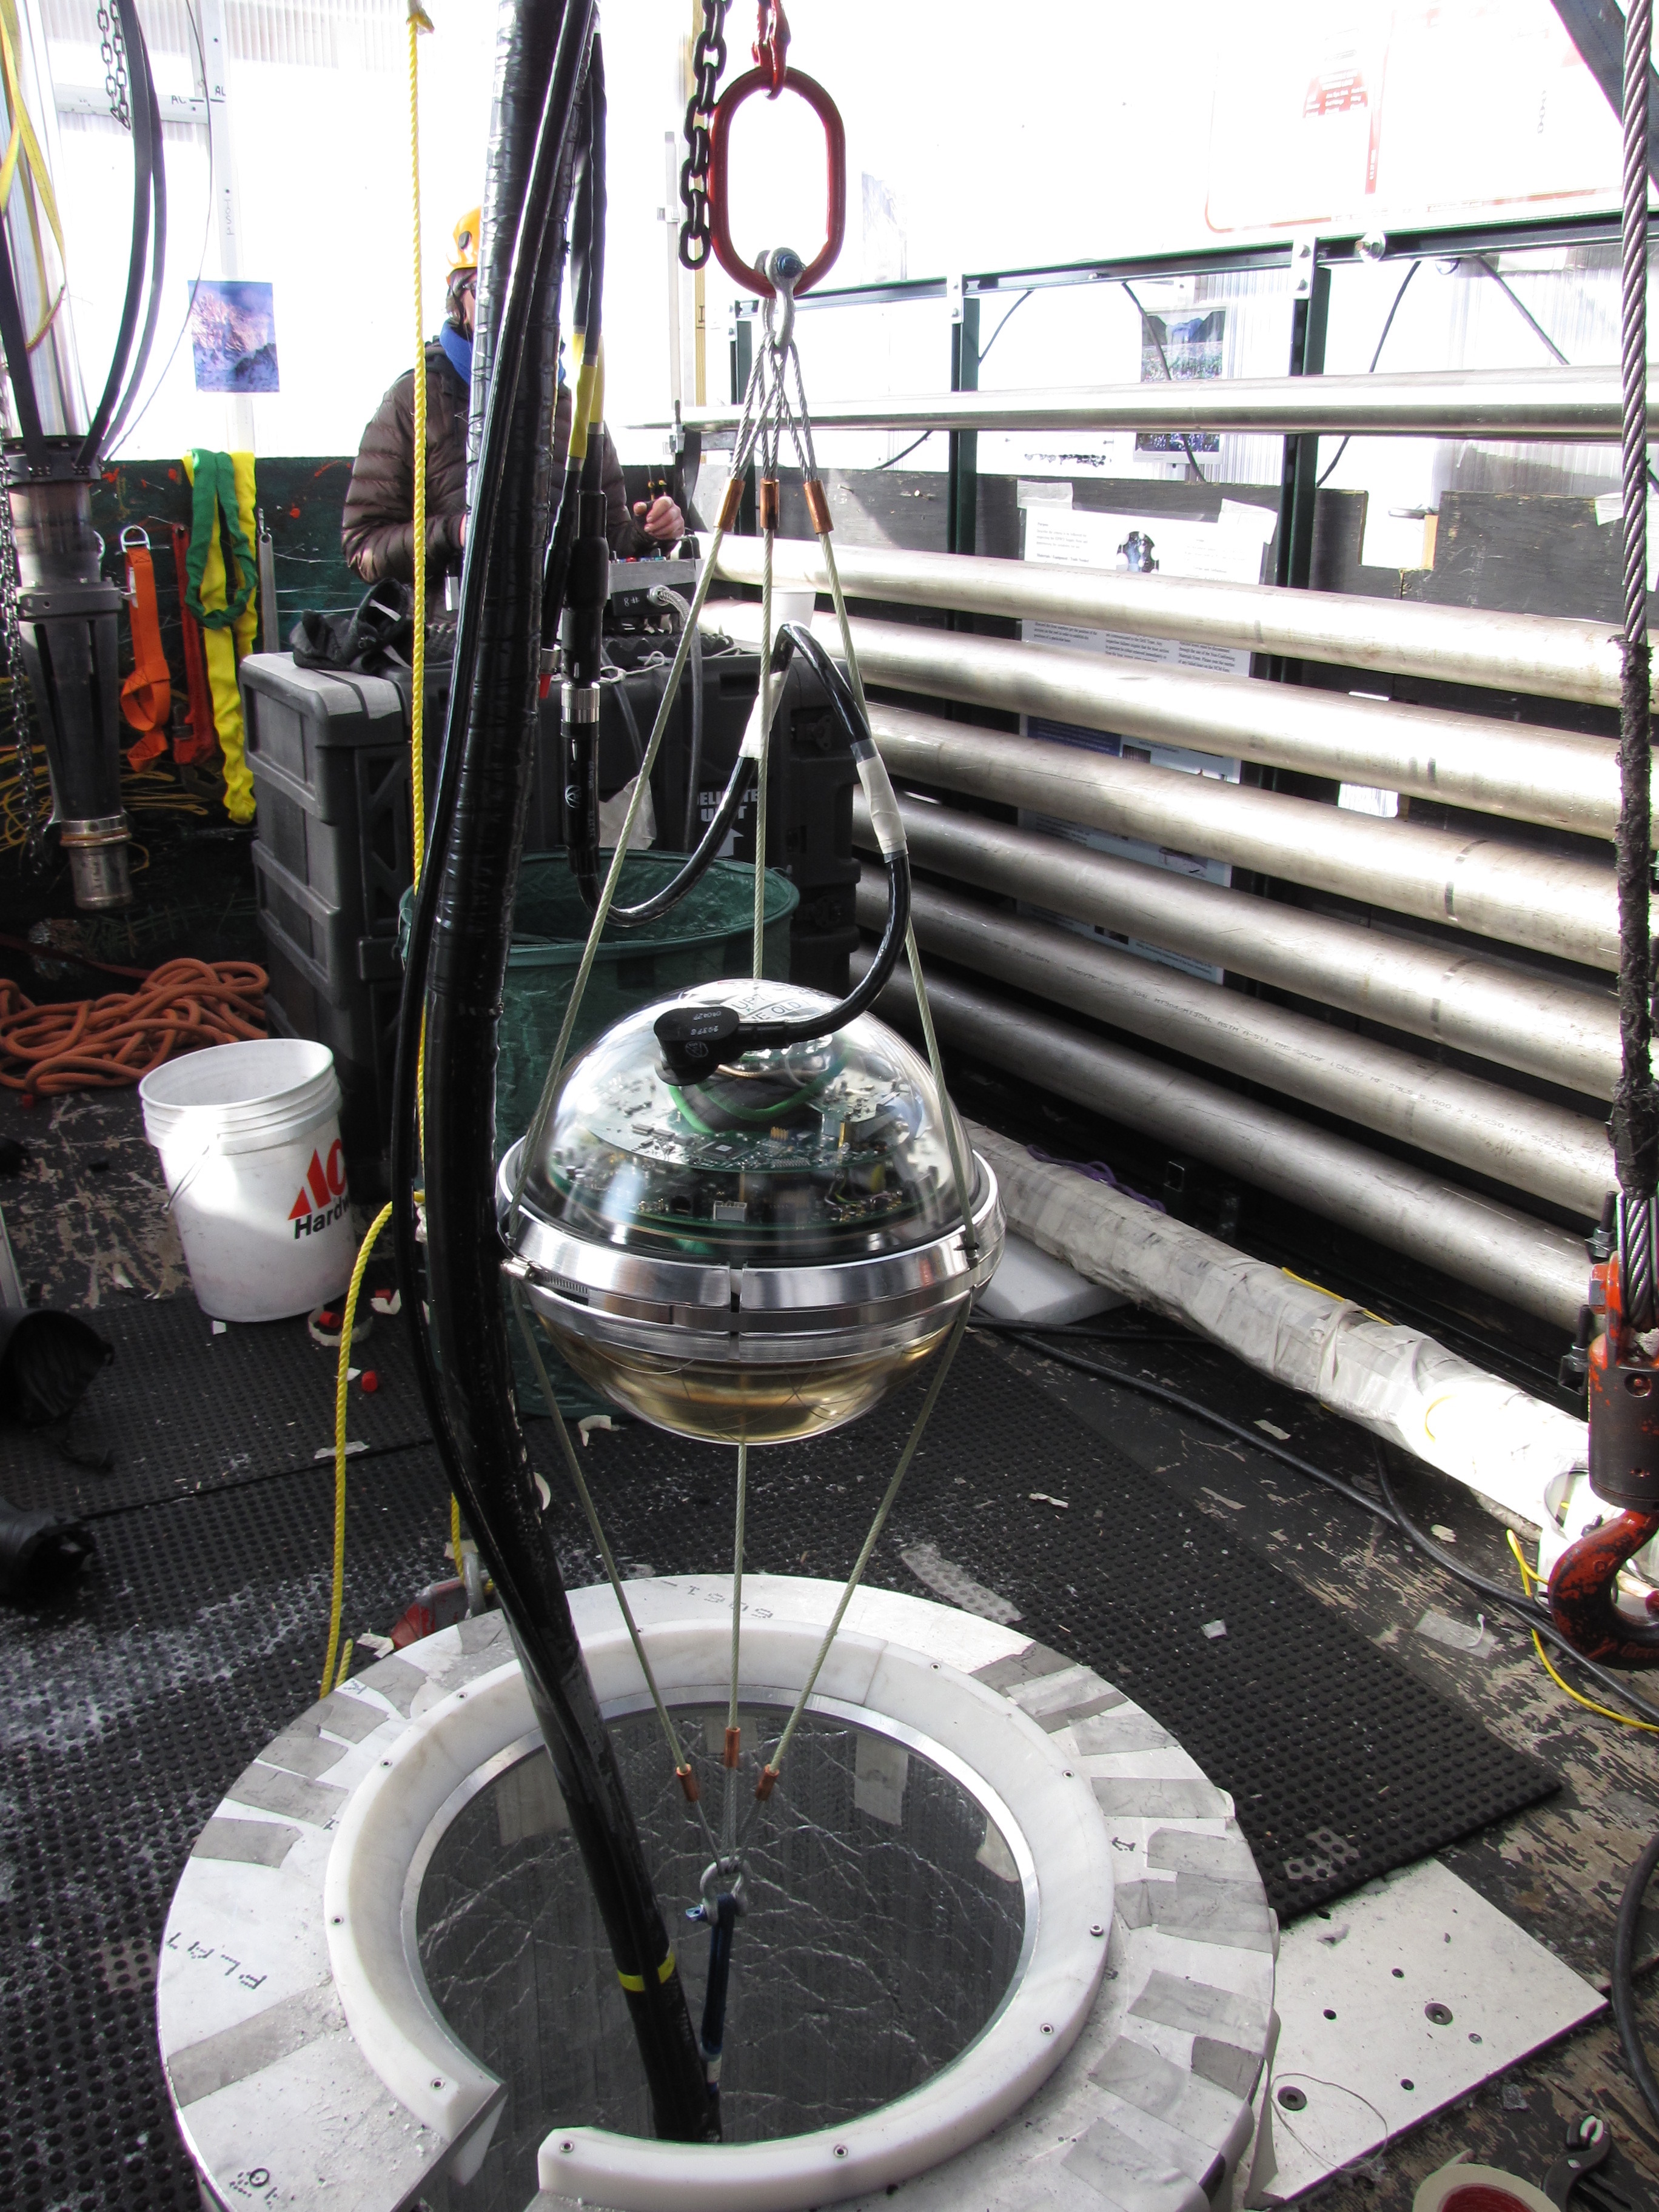
\includegraphics[width=0.35\textwidth]{img/dom-deployment-15-IMG_0080-652058109-3}}
  \caption{IceCube's optical module in relation to the main cable.}
  \label{fig:ahyoi7Ma}
\end{figure}

\subsubsection{Asymmetric Shadowing Effect Caused by the Cable}

Using the new medium-propagation algorithm, the cable can be simulated as one or several cylinders with limited $z$-range, which are configured for instant absorption.

As a first test, a simulation can be performed to verify that the cable causes an asymmetric shadowing effect, that is to say shields photons approaching photons from one direction while not shielding photons approaching from the opposite direction. Figure \ref{fig:ochoCh7o} shows the effective angular sensitivity of the optical module measured in such a simulation and confirms that the asymmetric shadowing can be observed in simulations.

\docpar{This simulation, placing an opaque cylinder part besides the optical module, propagating the photons with the hole-ice-correction algorithm (section \ref{sec:algorithm_a}) and scanning the effective angular acceptance, is documented in \issue{35}.}

\begin{figure}[htbp]
  \subcaptionbox{\steamshovel visualization of the simulation scenario. Photons approaching from different angles are either shielded by the cable or can reach the optical module unhindered.}{\halfimage{cable-shadow-steamshovel-commented}\vspace*{7mm}}\hfill
  \subcaptionbox{Effective angular acceptance of the optical module measured in the simulation. Photons approaching from the side of the cable are less likely to reach the optical module and be registered as a hit.}{\halfimage{cable-shadow-angular-acceptance-commented}}
  \caption{Simulation with the main cable modelled as opaque cylinder placed besides the optical module.}
  \label{fig:ochoCh7o}
\end{figure}

\subsubsection{Can the Cable Effect Account for the Observed Hole Ice Effects?}

% > mrongen [7:53 PM 2018-03-26]
% > Ok getting back to the bigger picture:
% > The overall state of observations IMHO only leaves us with three plausible true realizations:
% >  1. There is no bubble column
% >  2. It is (usually) small and centered around the DOM
% >  3. It is (usually) at the cable position
% >
% > These hypothesis (no bubble column being the null hypothesis against which the other two are tested) are actually fairly easy to test given the usual machinery. Use the new PPC with photon deletion on the cable, use direct detection (is that still in there?) and scan scattering length, size for both geometrical hypothesis (3 might need a small adjustment in PPC...) if the LLH improvement is significant that's it.
% >
% > A cross check for hypothesis 1 is also to see which scattering length (in a simulation without the cable and the column filling the entire drill hole) fits simulation data with the cable only. If it is 50cm that kind of explains why H2 has been so hard to kill (edited)


\url{https://github.com/fiedl/hole-ice-study/issues/101}


\cite{martinspicehddard}, slide 39:
> Currentcableimplementationdeletesphotonfrom
> a given range of azimuthal impact directions
> → cable is not allowed to be inside bubble